% =======================================================================================
\section{The Galactic-Binary Signal and the \acs{lisa} Response}
\label{app:forward-model}
% =======================================================================================

The forward model maps the $S=\ForwardModelSources{}$ sources of a window and the window's centre
frequency $\fw$ to the noiseless Fourier coefficients of the \ac{tdi} channels $A$, $E$ and $T$ on
the window's $K$ frequency bins. Each source's response is computed by JaxGB \citep{jaxgb}, a
differentiable implementation of the fast \ac{gb} response of \citet{cornish2007tests}, on the
equal-arm orbits of \acs{lisa}~Orbits \citep{lisaorbits}. The noise, the likelihood and the
\ac{snr} are in \cref{app:noise}, which also collects the checks of this model against published
references (\cref{app:noise-validation}); the priors are in \cref{app:priors} and the flow's
coordinates in \cref{app:chart}.

\subsection{Waveform}
\label{app:forward-model-waveform}

A detached compact binary in the Galaxy, most often a pair of white dwarfs, emits a
quasi-monochromatic \ac{gw} at twice its orbital frequency, which drifts slowly through
radiation reaction \citep{nelemans2001gravitational,korol2017prospects}. The
transverse-traceless strain of the plane wave is
\begin{equation}
  h_{ij}(\xi) = h_+(\xi)\,e^+_{ij} + h_\times(\xi)\,e^\times_{ij},\qquad
  \xi = t - \frac{\hat{\mathbf k}\cdot\mathbf x(t)}{c},
  \label{eq:forward-model-xi}
\end{equation}
with $\hat{\mathbf k}$ the direction of propagation, $\mathbf x$ the position of the observer and
$e^{+,\times}_{ij}$ the polarisation tensors of the source frame. For a circular binary with a
small, constant frequency derivative,
\begin{equation}
  h_+(\xi) = -\Amp\,\bigl(1+\cos^2\iota\bigr)\cos\Psi(\xi),\qquad
  h_\times(\xi) = -2\Amp\cos\iota\,\sin\Psi(\xi),\qquad
  \Psi(\xi) = -\phi_0 + 2\pi f_0\,\xi + \pi\fdot\,\xi^2,
  \label{eq:forward-model-waveform}
\end{equation}
with strain amplitude $\Amp$, frequency $f_0$, frequency derivative $\fdot$ and phase $\phi_0$, all
at the start of the observation, $t=0$. The inclination $\iota\in[0,\pi]$ is the angle between
the orbital angular momentum and the line of sight ($\iota=0$ face-on, $\pi/2$ edge-on, $\pi$
face-off); an isotropic orientation has $\cos\iota$ uniform (\cref{app:priors}).

The sky position (right ascension $\alpha$, declination $\delta$) in the equatorial
frame of the orbit files defines the orthonormal triad
\begin{equation}
  \hat{\mathbf u} = (\sin\alpha,\,-\cos\alpha,\,0),\qquad
  \hat{\mathbf v} = (-\sin\delta\cos\alpha,\,-\sin\delta\sin\alpha,\,\cos\delta),\qquad
  \hat{\mathbf k} = (-\cos\delta\cos\alpha,\,-\cos\delta\sin\alpha,\,-\sin\delta),
  \label{eq:forward-model-triad}
\end{equation}
and with it the polarisation tensors of the \ac{ssb},
$\epsilon^+_{ij} = (\hat{\mathbf u}\otimes\hat{\mathbf u} - \hat{\mathbf v}\otimes\hat{\mathbf v})_{ij}$
and
$\epsilon^\times_{ij} = (\hat{\mathbf u}\otimes\hat{\mathbf v} + \hat{\mathbf v}\otimes\hat{\mathbf u})_{ij}$.
The source frame is the \acs{ssb} frame rotated by the polarisation angle $\psi$,
$e^+_{ij} = \cos2\psi\,\epsilon^+_{ij} + \sin2\psi\,\epsilon^\times_{ij}$ and
$e^\times_{ij} = -\sin2\psi\,\epsilon^+_{ij} + \cos2\psi\,\epsilon^\times_{ij}$. In complex form,
$h_{ij}(\xi) = \mathrm{Re}\bigl\{\bigl(A_+\epsilon^+_{ij} + A_\times\epsilon^\times_{ij}\bigr)e^{\ii\Psi(\xi)}\bigr\}$ with
\begin{equation}
  A_+ = -\Amp\bigl[(1+\cos^2\iota)\cos2\psi + 2\ii\cos\iota\sin2\psi\bigr],\qquad
  A_\times = -\Amp\bigl[(1+\cos^2\iota)\sin2\psi - 2\ii\cos\iota\cos2\psi\bigr].
  \label{eq:forward-model-complex-amp}
\end{equation}
The sky prior is built in galactic coordinates and rotated to this equatorial frame
(\cref{app:priors}); sources quoted in ecliptic coordinates, as in the \acs{lisa} Data
Challenges, must be rotated to it as well.

\paragraph{Helicity form.}
In the circular basis $\epsilon^\pm_{ij} = (\epsilon^+_{ij} \pm \ii\epsilon^\times_{ij})/2$, the two
complex amplitudes of \cref{eq:forward-model-complex-amp} combine into
\begin{equation}
  A_+\epsilon^+_{ij} + A_\times\epsilon^\times_{ij}
  = -\Amp\Bigl[(1+\cos\iota)^2 e^{2\ii\psi}\,\epsilon^-_{ij} + (1-\cos\iota)^2 e^{-2\ii\psi}\,\epsilon^+_{ij}\Bigr],
  \label{eq:forward-model-helicity}
\end{equation}
so, with $e^{\ii\Psi}$ carrying $e^{-\ii\phi_0}$, the data depend on $(\Amp,\iota,\psi,\phi_0)$ only
through the two complex numbers $\Amp(1+\cos\iota)^2e^{-\ii(\phi_0-2\psi)}$ and
$\Amp(1-\cos\iota)^2e^{-\ii(\phi_0+2\psi)}$. A face-on or face-off source carries only one of them,
and its $\psi$ and $\phi_0$ enter only through one combination $\phi_0\mp2\psi$. Both numbers are
invariant under the symmetries of \cref{eq:psi-phi-symmetry}. The flow's helicity amplitudes
$z_\pm$ (\cref{eq:chart}) are these two numbers, rescaled.

\paragraph{Chirp.}
For a circular binary driven by gravitational radiation alone, the frequency derivative is
fixed by the chirp mass $\Mc$,
\begin{equation}
  \fdot = \frac{96}{5}\,\pi^{8/3}\left(\frac{G\Mc}{c^3}\right)^{5/3} f_0^{11/3}.
  \label{eq:forward-model-fdot}
\end{equation}
Each source is parametrised by $\theta = (f_0, \Mc, \Amp, \alpha, \delta, \psi, \iota, \phi_0)$, and
the response is evaluated with $\fdot$ from \cref{eq:forward-model-fdot}. The amplitude is a free
parameter rather than a function of $\Mc$, $f_0$ and the distance; its prior is set through each
source's own \ac{snr} (\cref{app:priors}). Tides and mass transfer, which change $\fdot$ for some
systems, are neglected.

\paragraph{Phase reference.}
The response takes $\phi_0$ at the start of the observation; the flow coordinates
(\cref{app:chart}) use the phase at mid-observation,
\begin{equation}
  \phi_0^{\rm mid} = \phi_0 - \pi f_0\Tobs - \tfrac{\pi}{4}\fdot\,\Tobs^2 = -\Psi\bigl(\Tobs/2\bigr),
  \label{eq:forward-model-phase-mid}
\end{equation}
which ignores the $\hat{\mathbf k}\cdot\mathbf x/c$ term of $\xi$. A change $\delta f_0$ rotates the
phase at time $t$ by $2\pi\,\delta f_0\,t$; measured from mid-observation these rotations cancel on
average, so the posterior of $\phi_0^{\rm mid}$ is close to uncorrelated with $f_0$, whereas the
start phase inherits a strong correlation with it. It is not decorrelated from $\fdot$: since
$f_0$ is the frequency at the start, a change of $\fdot$ also moves the frequency at
mid-observation.

\subsection{Single-Link Response}
\label{app:forward-model-link}

\ac{lisa} measures the wave as relative frequency fluctuations of six laser links between three
spacecraft. Let $i$ be the receiving and $j$ the emitting spacecraft of link $ij$, $t_i$ the
time of reception and $t_j = t_i - L_{ij}(t_i)$ the time of emission, with $L_{ij}$ the light
travel time. The link response is \citep{finn2009response,cornish2009alternative}
\begin{equation}
  y_{ij}(t_i) = -\frac12\,\frac{H_{ij}(\xi_i) - H_{ij}(\xi_j)}{1 - \hat{\mathbf k}\cdot\hat{\mathbf x}_{ij}},
  \qquad
  H_{ij}(\xi) = \hat x^k_{ij}\hat x^l_{ij}\,h_{kl}(\xi),
  \label{eq:forward-model-link}
\end{equation}
with $\xi_i = t_i - \hat{\mathbf k}\cdot\mathbf x_i(t_i)/c$,
$\xi_j = t_j - \hat{\mathbf k}\cdot\mathbf x_j(t_j)/c$, and $\hat{\mathbf x}_{ij}$ the unit vector
from the emitter to the receiver; \acs{lisa}~\acs{gw}~Response \citep{lisagwresponse} uses the same
response, triad and polarisation convention. For the \ac{gb}, let
$\mathcal A_{ij} = A_+F^+_{ij} + A_\times F^\times_{ij}$, with the antenna patterns
$F^+_{ij} = (\hat{\mathbf u}\cdot\hat{\mathbf x}_{ij})^2 - (\hat{\mathbf v}\cdot\hat{\mathbf x}_{ij})^2$
and $F^\times_{ij} = 2(\hat{\mathbf u}\cdot\hat{\mathbf x}_{ij})(\hat{\mathbf v}\cdot\hat{\mathbf x}_{ij})$, and
\begin{equation}
  \alpha_{ij}(t_i) = \pi L_{ij}\,\bigl(1 - \hat{\mathbf k}\cdot\hat{\mathbf x}_{ij}\bigr)\,
  \bigl(f_0 + \fdot\,\xi_i\bigr),
  \label{eq:forward-model-alpha}
\end{equation}
half the phase the wave advances along the link. If the frequency does not change
appreciably during one light travel time,
\begin{equation}
  y_{ij}(t_i) = -\mathrm{Re}\left\{\frac{\ii\,\mathcal A_{ij}\sin\alpha_{ij}}
  {1 - \hat{\mathbf k}\cdot\hat{\mathbf x}_{ij}}\,
  e^{-\ii\left(\alpha_{ij} - \Psi(\xi_i)\right)}\right\}.
  \label{eq:forward-model-link-gb}
\end{equation}
We make two further approximations: the emitter's position is taken at the time of reception,
$\mathbf x_j(t_j)\simeq\mathbf x_j(t_i)$, so that $\hat{\mathbf x}_{ji} = -\hat{\mathbf x}_{ij}$ and
$\mathcal A_{ji} = \mathcal A_{ij}$; and all six light travel times are equal and constant,
$L_{ij} = L = \qty{\ForwardModelArmGm}{\giga\metre}/c = \qty{\ForwardModelArmSeconds}{\second}$, which puts the
transfer frequency at $f_\star = (2\pi L)^{-1} = \qty{\ForwardModelFStar}{\milli\hertz}$.

\subsection{Heterodyned Frequency-Domain Response}
\label{app:forward-model-heterodyne}

With $q = \operatorname{rint}(f_0\Tobs)$ the frequency bin nearest to $f_0$, the response separates
into a carrier and a slowly varying envelope,
$y_{ij}(t) = \mathrm{Re}\bigl\{\mathcal G_{ij}(t)\,e^{2\pi\ii qt/\Tobs}\bigr\}$, with
\begin{equation}
  \mathcal G_{ij}(t) = -\frac{\ii}{2}\,\frac{f_0 + \fdot\,\xi_i}{f_{\star}}\,\mathcal A_{ij}\,
  \operatorname{sinc}\alpha_{ij}\;
  \exp\Bigl\{-\ii\Bigl[\alpha_{ij} + 2\pi f_0\frac{\hat{\mathbf k}\cdot\mathbf x_i(t)}{c}
  - \Bigl(-\phi_0 + 2\pi\bigl(f_0 - \tfrac{q}{\Tobs}\bigr)t + \pi\fdot\,\xi_i^2\Bigr)\Bigr]\Bigr\},
  \label{eq:forward-model-slow}
\end{equation}
where $\operatorname{sinc}x = \sin x/x$; this is \cref{eq:forward-model-link-gb} with the carrier
taken out, since
$\tfrac12(f/f_\star)\operatorname{sinc}\alpha_{ij} = \sin\alpha_{ij}/(1-\hat{\mathbf k}\cdot\hat{\mathbf x}_{ij})$.
The envelope is sampled at the $R$ times $t_m = m\Tobs/R$, $m = 0,\dots,R-1$, and
Fourier-transformed with a rectangular window, which gives the positive-frequency spectrum on
the $R$ bins starting at $k_{\min} = q - R/2$:
\begin{equation}
  \tilde y_{ij}\Bigl(\frac{q+k}{\Tobs}\Bigr) = \frac{\Tobs}{2R}\sum_{m=0}^{R-1}\mathcal G_{ij}(t_m)\,
  e^{-2\pi\ii km/R},\qquad k = -\tfrac R2,\dots,\tfrac R2 - 1.
  \label{eq:forward-model-heterodyne}
\end{equation}
We call $R$ the number of response points. The prefactor makes this the positive-frequency half
of the continuous Fourier transform $\int_0^{\Tobs}h(t)\,e^{-2\pi\ii ft}\,\dd t$; the noise is
normalised to match (\cref{app:noise-likelihood}), so no sampling cadence enters any \ac{snr}.
The negative-frequency lobe is not folded in, so every source needs $k_{\min}\ge0$, which both
bands satisfy with a wide margin.

\paragraph{Bandwidth of the envelope.}
The envelope varies on the time scale of \acs{lisa}'s orbit, so its spectrum is confined to a band of
bins around $q$. That band holds three contributions: the annual Doppler sideband,
$\pm f_0v_\oplus/c$, with $v_\oplus = \qty{\ForwardModelVelocity}{\kilo\metre\per\second}$, so
$v_\oplus/c\simeq\num{\ForwardModelVelocityRatio}$; the chirp drift $\fdot\,\Tobs$; and the sidebands of the
antenna pattern, which rotates with the constellation's yearly orbit and modulates the signal at
harmonics of $1/\unit{\year}$ up to the \ForwardModelAntennaOrdinal{} \citep{cutler1998angular}. A source
therefore needs
\begin{equation}
  n_{\rm span}(f_0,\Mc) = 2\left\lceil\Bigl(\frac{f_0 v_\oplus}{c}
  + \fdot(\Mc, f_0)\,\Tobs + \frac{\ForwardModelAntennaHarmonics{}}{\unit{\year}}\Bigr)\Tobs\right\rceil \le R
  \label{eq:forward-model-span}
\end{equation}
bins, with $\Tobs = \qty{\ForwardModelTobsYears}{\year}$ and bins of width
$1/\Tobs = \qty{\ForwardModelBinNanoHz}{\nano\hertz}$; the antenna term alone is \ForwardModelAntennaBins{} bins.
The Doppler term is linear in $f_0$ and the chirp term grows as $f_0^{11/3}$. For the heaviest
binary in the prior, $\Mc_{\max} = \ForwardModelMassMax{}\cdot2^{-1/5}\,\unit{\solarmass} = \qty{\ForwardModelMcMax}{\solarmass}$
(an equal-mass pair at the top of the mass range), the chirp overtakes the Doppler sideband
above about \qty{\ForwardModelChirpCross}{\milli\hertz}, and from there quadrupling $R$ extends the reachable band
by a factor of only $4^{3/11}\simeq\ForwardModelQuadruple{}$ (\cref{fig:forward-model}a).

\paragraph{Truncation.}
\Cref{eq:forward-model-span} bounds where the envelope's power lies, not all of it. A
rectangular window spreads a tone that falls between two bins into a Dirichlet kernel whose
tails decay only as $1/k$, and the $R$-point transform folds the tails beyond $\pm R/2$ back onto
the $R$ bins. The $R$-bin response therefore keeps a source's power but not the exact shape of
its spectrum. \Cref{tab:forward-model-truncation} compares it with a
\num{\ForwardModelReferencePoints}-point response for sources drawn from each band's prior. The error
is set by leakage, not by the span: it is small for a source on a bin centre and largest halfway
between two bins (\cref{fig:forward-model}b), while the reference holds almost none of its power
outside the $R$ bins. Over a ladder of $R$ it falls as $R^{\ForwardModelNarrowLadderSlope{}}$ (narrow)
and $R^{\ForwardModelFullLadderSlope{}}$ (full), close to the $R^{-1/2}$ of a $1/k$ tail
(\cref{fig:forward-model}c). Each source's \ac{snr} is preserved, but the residual between the two
responses is not small against the noise, so the data of a loud source are distinguishable from
a full-resolution transform of the same signal. Training, the test injections and the reference
\ac{mcmc} all use the same $R$-bin response, so the comparison between the flow and the \ac{mcmc}
is unaffected (\cref{app:forward-model-limits}).

\begin{table}[h]
\caption{The $R$-bin response against a \num{\ForwardModelReferencePoints}-point reference, for
\num{\ForwardModelNarrowTruncSources} sources from each band's prior. Errors are the relative $L_2$
difference of a source's $A$, $E$, $T$ coefficients; on- and off-bin are the tenth of sources
nearest a bin centre and nearest halfway between two bins; $\snr_{\rm res}$ is the \acs{snr} of the
difference.}
\label{tab:forward-model-truncation}
\centering
\small
\begin{tabular}{lrrrrrrrr}
\toprule
band & $R$ & median & max & on-bin & off-bin & power outside $R$ & $\snr_{\rm res}$ median & $\snr_{\rm res}>1$ \\
\midrule
narrow & \ForwardModelNarrowR{} & \qty{\ForwardModelNarrowTruncRelMedian}{\percent} & \qty{\ForwardModelNarrowTruncRelMax}{\percent} & \qty{\ForwardModelNarrowTruncRelOnBin}{\percent} & \qty{\ForwardModelNarrowTruncRelOffBin}{\percent} & $\le$\qty{\ForwardModelNarrowTruncOutsideMax}{\percent} & \ForwardModelNarrowTruncRhoResMedian{} & \qty{\ForwardModelNarrowTruncRhoResOverOne}{\percent} \\
full & \ForwardModelFullR{} & \qty{\ForwardModelFullTruncRelMedian}{\percent} & \qty{\ForwardModelFullTruncRelMax}{\percent} & \qty{\ForwardModelFullTruncRelOnBin}{\percent} & \qty{\ForwardModelFullTruncRelOffBin}{\percent} & $\le$\qty{\ForwardModelFullTruncOutsideMax}{\percent} & \ForwardModelFullTruncRhoResMedian{} & \qty{\ForwardModelFullTruncRhoResOverOne}{\percent} \\
\bottomrule
\end{tabular}
\end{table}

\begin{figure}[t]
  \centering
  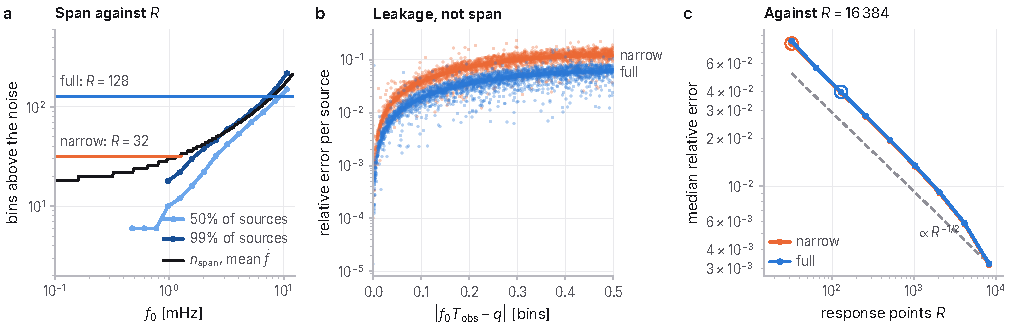
\includegraphics[width=\textwidth]{figures/forward-model.pdf}
  \caption{Choosing $R$ and what it costs. (a) The half-span of the heaviest binary's response,
  $\Mc = \qty{\ForwardModelMcMax}{\solarmass}$ (\cref{eq:forward-model-span}), and its three terms, against
  each band's $R/2$: above a few \unit{\milli\hertz} the chirp dominates, and the dots mark the highest $f_0$ each
  $R$ holds (\qtylist{\ForwardModelNarrowHolds;\ForwardModelFullHolds}{\milli\hertz}). (b) Each source's relative
  error against a \num{\ForwardModelReferencePoints}-point response grows with its distance from a bin
  centre: the error is leakage of the rectangular window, not lost span. (c) The median error
  over a ladder of $R$ falls close to $R^{-1/2}$; rings mark each band's own $R$.}
  \label{fig:forward-model}
\end{figure}

\subsection{Time-Delay Interferometry}
\label{app:forward-model-tdi}

Laser frequency noise is cancelled by \ac{tdi} \citep{tinto2021time}. For equal and constant arms,
the Michelson combinations are formed on the envelopes of \cref{eq:forward-model-slow}, with the
instantaneous frequency $f = f_0 + \fdot\,t$ and the delay phase $x = 2\pi fL = f/f_\star$:
\begin{equation}
  X = -2\ii\sin x\;e^{-\ii x}\Bigl[\bigl(\mathcal G_{21} - \mathcal G_{31}\bigr)
  + e^{-\ii x}\bigl(\mathcal G_{12} - \mathcal G_{13}\bigr)\Bigr],
  \label{eq:forward-model-tdi-x}
\end{equation}
with $Y$ and $Z$ from the cyclic permutation $1\to2\to3\to1$, Fourier-transformed as in
\cref{eq:forward-model-heterodyne}. This is \acs{tdi} generation 1.5, which the noise model of
\cref{app:noise} assumes; generation 2 would multiply every channel by
$1 - e^{-4\ii x} = 2\ii\sin2x\,e^{-2\ii x}$ and the noise \ac{psd} by the matching $4\sin^22x$.

Since $-2\ii\sin x\,e^{-\ii x} = -(1 - D^2)$ with $D = e^{-\ii x}$ the delay operator,
\cref{eq:forward-model-tdi-x} is $(1-D^2)$ times a combination of the four links that involve
spacecraft 1. The standard equal-arm combination \citep[eq.~14]{babak2021lisa} pairs the delays
the other way round, $(1-D^2)\bigl[(y_{13}-y_{12}) + D\,(y_{31}-y_{21})\bigr]$; the two differ by
$(1-D^2)(1-D)\bigl[(y_{13}-y_{31}) - (y_{12}-y_{21})\bigr]$, which is of higher order in $x$.
On the same link responses the difference indeed grows as $f_0^3$ and stays below a percent
over the band (\cref{app:noise-validation}, \cref{fig:forward-model-checks}a). The channels are
the quasi-orthogonal combinations \citep{prince2002lisa}
\begin{equation}
  A = \frac{Z-X}{\sqrt2},\qquad E = \frac{X-2Y+Z}{\sqrt6},\qquad T = \frac{X+Y+Z}{\sqrt3},
  \label{eq:forward-model-aet}
\end{equation}
whose noises are uncorrelated for equal arms (\cref{app:noise}).

\subsection{Frequency Windows}
\label{app:forward-model-windows}

A training example is one window of $K = \ForwardModelWindowResponses{}R$ consecutive bins of the
$\Tobs$-long transform, identified by its centre frequency $\fw$, which every example carries with
its data. The first bin is
\begin{equation}
  k_0(\fw) = \ForwardModelWindowStride{}\,\operatorname{rint}\Bigl(\frac{\fw\Tobs - K/2}{\ForwardModelWindowStride{}}\Bigr),
  \label{eq:forward-model-window-start}
\end{equation}
so windows start on even bins and $\fw = (k_0 + K/2)/\Tobs$ exactly for the centres the sampler
produces. The window holds $S$ sources, whose $R$-bin responses are added at their offsets
$k_{\min} - k_0$; overlapping sources add linearly. A guard band of $R/2$ bins at each edge keeps
every response inside the window: sources are drawn with
\begin{equation}
  f_0 \in \Bigl[\max\Bigl(\frac{k_0 + R/2}{\Tobs}, f_{\min}\Bigr),\;
          \min\Bigl(\frac{k_0 + K - R/2}{\Tobs}, f_{\max}\Bigr)\Bigr],
  \label{eq:forward-model-window-interior}
\end{equation}
an interior of $\ForwardModelInteriorResponses{}R$ bins, and since a response spans $q\pm R/2$ it ends
at the window's edge at most. The centre is drawn by sampling $f_c$ log-uniformly on
$[f_{\min}, f_{\max}]$, snapping it to the grid of \cref{eq:forward-model-window-start} and
clipping the window index to the range whose interiors just cover $[f_{\min}, f_{\max}]$, so
windows follow the $1/f_0$ density of the frequency prior (\cref{app:priors}) up to the snapping
and the clipped ends.

\Cref{fig:forward-model-window} shows one window of each band as the network receives it. Per
bin, the sources are mostly below the noise: a source's \acs{snr} accumulates over its whole
span, so even a loud one is barely visible in the raw data of the full band, where its power is
spread over hundreds of bins.

\begin{figure}[t]
  \centering
  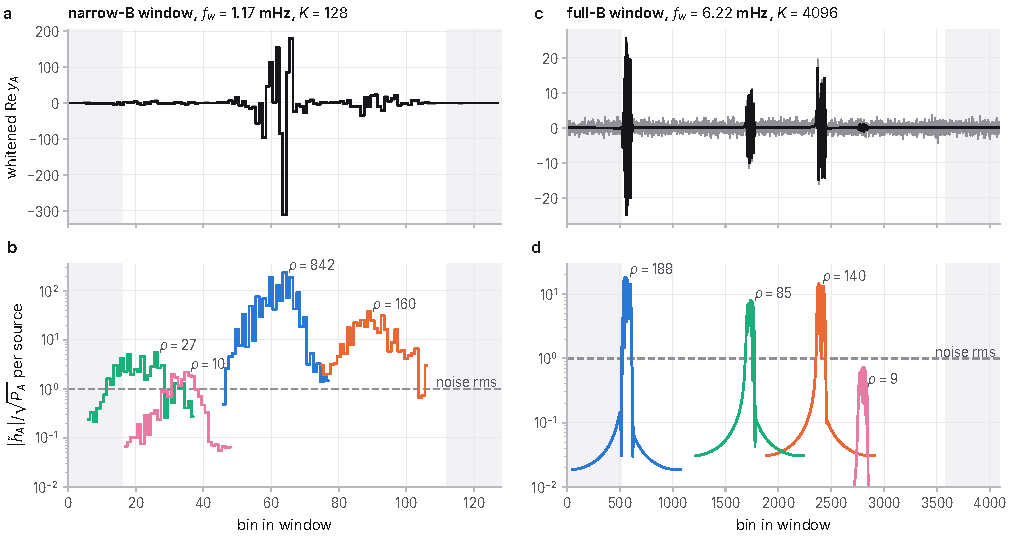
\includegraphics[width=\textwidth]{figures/training-window.pdf}
  \caption{One training window per band, drawn from the prior. (a, b) The network's input in the
  real part of channel $A$ (\cref{eq:noise-whiten}; grey) with the noiseless signal whitened the
  same way (black); the noise has unit variance. (c, d) Each source's $A$ response alone, in
  units of the noise's rms per bin, labelled with its \acs{snr}; shading marks the guard bands,
  which hold no $f_0$, only the responses' wings. A narrow-band response covers a few bins around
  $f_0$; at high frequency on the full band the Doppler and chirp terms spread it over hundreds,
  each bin well below the noise.}
  \label{fig:forward-model-window}
\end{figure}

\paragraph{Bands.}
The problem comes in two bands that share every prior and the window layout and differ only in
$f_{\max}$, and with it $R$ (\cref{tab:forward-model-bands}). Given the band, $R$ is the power of two
at or above $n_{\rm span}(f_{\max},\Mc_{\max})$; conversely, for a given $R$ the highest admissible
$f_0$ is the largest one with $n_{\rm span}(f_0,\Mc_{\max})\le R$. On the full band, at
\qty{\ForwardModelFullTop}{\milli\hertz} the Doppler sideband is \ForwardModelFullDoppler{} bins, the chirp of the
heaviest binary \ForwardModelFullChirp{} and the antenna sidebands \ForwardModelAntennaBins{}, so
$n_{\rm span} = \ForwardModelFullSpan{}$ and $R = \ForwardModelFullR{}$, which would hold the heaviest
binaries up to \qty{\ForwardModelFullHolds}{\milli\hertz}. The narrow band stops at \qty{\ForwardModelNarrowTop}{\milli\hertz}, where
the Doppler sideband is \ForwardModelNarrowDoppler{} bins and the chirp \ForwardModelNarrowChirp{}, so
$n_{\rm span} = \ForwardModelNarrowSpan{} = R$ fills its response exactly.

\begin{table}[h]
\caption{The two bands. They share the priors, the \ForwardModelSourcesWord{} sources per window
and the window layout; $R$, the window and the number of distinct windows differ. The band
fraction is of $\log f_0$ over \qtyrange{\ForwardModelBandLow}{\ForwardModelBandHigh}{\milli\hertz}.}
\label{tab:forward-model-bands}
\centering
\small
\begin{tabular}{lrrrrlr}
\toprule
band & $R$ & window $K$ & interior & windows & $f_0$ range & band fraction \\
\midrule
narrow & \ForwardModelNarrowR{} & \ForwardModelNarrowK{} & \ForwardModelNarrowInterior{} & \num{\ForwardModelNarrowWindows} & \qtyrange{\ForwardModelNarrowLow}{\ForwardModelNarrowTop}{\milli\hertz} & \qty{\ForwardModelNarrowFraction}{\percent} \\
full & \ForwardModelFullR{} & \ForwardModelFullK{} & \ForwardModelFullInterior{} & \num{\ForwardModelFullWindows} & \qtyrange{\ForwardModelFullLow}{\ForwardModelFullTop}{\milli\hertz} & \qty{\ForwardModelFullFraction}{\percent} \\
\bottomrule
\end{tabular}
\end{table}

\subsection{What the Simulator Leaves Out}
\label{app:forward-model-limits}

The training distribution is deliberately simpler than real \acs{lisa} data.
\begin{itemize}
  \item Every window holds exactly \ForwardModelSourcesWord{} resolvable binaries and nothing else:
  no confusion foreground from the unresolved binaries
  \citep{timpano2006characterizing,karnesis2021characterization}, no other source class, and no
  source that straddles a window edge or leaks in from a neighbouring window.
  \item The noise is stationary, Gaussian and known (\cref{app:noise}), without gaps or glitches.
  \item The constellation has equal, constant arms, the emitter's position is taken at
  reception, and \acs{tdi} is the equal-arm generation 1.5.
  \item The frequency evolves by gravitational radiation alone, with a constant $\fdot$ fixed by
  $\Mc$: no $\ddot f$, tides or mass transfer.
  \item Each source's response is cut to its $R$ bins (\cref{tab:forward-model-truncation}).
\end{itemize}
The same simulator generates the training data, the test injections and the likelihood of the
reference \ac{mcmc} (\cref{app:mcmc}), so these simplifications affect realism, not the consistency
of the comparison. Using the posteriors inside a global fit would require lifting the first: a
variable number of sources per window, and sources that straddle window edges.
